\documentclass[letterpaper,12pt,titlepage,oneside,final]{book}

\title{Automating Programming Assignment Marking with AST Analysis}
\author{Stephen Li}
\date{} % TODO Update to date of presentation

%----------------------------------------------------------------------
% Settings and Packages
%----------------------------------------------------------------------

\usepackage[toc,page]{appendix} % Set up appendix
\usepackage{mathtools,amsmath,amssymb,amstext} % Lots of math symbols and environments
\usepackage{lipsum} % Generating dummy text to test out layout
\usepackage[labelfont=bf]{caption} % Bold caption's "Figure x"
\usepackage{multirow} % Allow table cell to span multiple rows
\usepackage{makecell} % Allow multirow cells with linebreaks
\usepackage{arydshln} % Dotted lines in table
\usepackage{colortbl} % Coloured lines in table
\usepackage{float} % Prevent figures/tables from floating out of place
\usepackage{listings} % For code blocks
\usepackage{booktabs} % For stylzing tables
\usepackage{csquotes} % For stylzing quotes
\usepackage{courier} % For courier font in code listing
\usepackage[group-separator={,}]{siunitx}
\usepackage{commath} % For abs symbols

% For including graphics
\usepackage[pdftex]{graphicx}
\graphicspath{ {../media/img/} }

% For drawing tikz diagrams
\usepackage{tikz}
\usetikzlibrary{shapes,arrows.meta,fit,positioning}

% Space before footnote's bar
\setlength{\skip\footins}{2cm}

% Useful utilities
\usepackage{etoolbox}

% CHANGE THIS VALUE TO "true" as necessary, to improve printed results for hard copies
% by overriding some options of the hyperref package below.
\newbool{PrintVersion}
\boolfalse{PrintVersion}

\newbool{IsPHD}
\boolfalse{IsPHD}

% Load this package last because it overrides other packages' properties
\usepackage[pdftex]{hyperref}
\hypersetup{
pdftitle={},
pdfauthor={},
    %------------------------
    plainpages=false,       % needed if Roman numbers in frontpages
    unicode=false,          % non-Latin characters in Acrobat’s bookmarks
    pdftoolbar=true,        % show Acrobat’s toolbar?
    pdfmenubar=true,        % show Acrobat’s menu?
    pdffitwindow=false,     % window fit to page when opened
    pdfstartview={FitH},    % fits the width of the page to the window
    pdfnewwindow=true,      % links in new window
    colorlinks=true,        % false: boxed links; true: colored links
    }

% For improved print quality, change some hyperref options
\ifbool{PrintVersion}{
\hypersetup{
        citecolor=black, % color of links to bibliography
        filecolor=black, % color of file links
        linkcolor=black, % color of internal links
        urlcolor=black   % color of external links
        }
        }{
        \hypersetup{
        citecolor=green,
        filecolor=magenta,
        linkcolor=blue,
        urlcolor=cyan
        }
        }

% Source code
\lstset{
, aboveskip = 2em
, frame = single
, basicstyle = \ttfamily\footnotesize
, numbers = left
, stepnumber = 1
, escapechar = !
}

% For frontmatter page headings that don't count as sections
\newcommand{\miniheading}[1]{\begin{center}\textbf{#1}\end{center}}

% Space between each paragraph
\setlength{\parskip}{\bigskipamount}

% Space between table caption text and other text
\captionsetup[table]{belowskip=2em}

% Space under table
\setlength{\textfloatsep}{4em}

% Indent for table's labels
\newcommand{\tspace}{\hspace{0.5cm}}

% How high each line is
\renewcommand{\baselinestretch}{1.2}

% Change table cell padding
\renewcommand{\arraystretch}{1.2}

% Booktabs table rules without padding
\newcommand{\Toprule}{\specialrule{\heavyrulewidth}{\abovetopsep}{0pt}}
\newcommand{\Bottomrule}{\specialrule{\heavyrulewidth}{0pt}{\belowbottomsep}}
\newcommand{\Midrule}{\specialrule{\lightrulewidth}{0pt}{0pt}}

% Space below figure caption
\captionsetup[figure]{belowskip=2em}

% By default, each chapter will start on a recto (right-hand side)
% page.  We also force each section of the front pages to start on
% a recto page by inserting \cleardoublepage commands.
% In many cases, this will require that the verso page be
% blank and, while it should be counted, a page number should not be
% printed.  The following statements ensure a page number is not
% printed on an otherwise blank verso page.
\let\origdoublepage\cleardoublepage
\newcommand{\clearemptydoublepage}{\clearpage{\pagestyle{empty}\origdoublepage}}
\let\cleardoublepage\clearemptydoublepage

% Automatically center figures/tables
\makeatletter
\g@addto@macro\@floatboxreset\centering
\makeatother

\begin{document}

%------------------------------------------------------------------------------
% Front Matter
%------------------------------------------------------------------------------

% The title page is counted as page `i' but we need to suppress the
% page number. Also, we don't want any headers or footers.
\pagestyle{empty}
\pagenumbering{roman}

\makeatletter
\begin{titlepage}
    \begin{center}
        \vspace*{1.0cm}

        \Huge
        {\@title}

        \vspace*{1.0cm}

        \normalsize
        by \\

        \vspace*{1.0cm}

        \Large
        \@author

		\vspace*{\fill}

        \normalsize
        A thesis \\
        presented to the University of Waterloo \\
        in fulfillment of the \\
        thesis requirement for the degree of \\
        Master of Mathematics \\
        in \\
        Computer Science \\

        \vspace*{2.0cm}

        Waterloo, Ontario, Canada, 2018 \\

        \vspace*{1.0cm}

        \copyright\ \@author \ 2018 \\
    \end{center}
\end{titlepage}
\makeatother

% The rest of the front pages should contain no headers and be numbered using Roman numerals starting with `ii'
\pagestyle{plain}
\setcounter{page}{2}

\cleardoublepage

% Required for Ph.D. theses only

\ifbool{IsPHD}{

% Use longest text to define tab length
\newenvironment{CommitteeTabbing}[1][\hspace{1.5in} \= ]
    {\begin{tabbing}#1\kill}
    {\end{tabbing}}

\miniheading{Examining Committee Membership}

\noindent
The following served on the Examining Committee for this thesis. The decision of the Examining Committee is by majority vote.

\bigskip

\noindent
\begin{CommitteeTabbing}
External Examiner:
\> John Smith \\
\> Professor, Dept. of Philosophy, University of Waterloo \\
\end{CommitteeTabbing}
\bigskip

\noindent
\begin{CommitteeTabbing}
Supervisors:
\> John Smith \\
\> Professor, Dept. of Philosophy, University of Waterloo \\
\\
\> Jane Doe \\
\> Professor, Dept. of Philosophy, University of Waterloo \\
\end{CommitteeTabbing}
\bigskip

\noindent
\begin{CommitteeTabbing}
Internal Member:
\> John Smith \\
\> Professor, Dept. of Philosophy, University of Waterloo \\
\end{CommitteeTabbing}
\bigskip

\noindent
\begin{CommitteeTabbing}
Other Members:
\> John Smith \\
\> Professor, Dept. of Philosophy, University of Waterloo \\
\end{CommitteeTabbing}
\bigskip

}{} % \ifbool{IsPHD}

\cleardoublepage

\noindent
I hereby declare that I am the sole author of this thesis. This is a true copy of the thesis, including any required final revisions, as accepted by my examiners.

\noindent
I understand that my thesis may be made electronically available to the public.

\cleardoublepage

\miniheading{Abstract}

This thesis presents a novel approach to automatically mark programming assignments. We hypothesize that correct student solution ASTs will be more similar to reference solution ASTs than incorrect student solutions and that their similarities can be quantitatively measured. Our approach first preprocesses the ASTs before computing their tree edit distances. We then aggregate the student's set of edit distances from every reference solution into a final mark for the student. We have implemented our approach in our ClangAutoMarker tool. Our experiments demonstrate promising potential for reducing a human marker's workload but further refinements are needed before its accuracy can be suitable for a live classroom.

\cleardoublepage

\miniheading{Acknowledgements}

I would like to thank my adviser Patrick Lam for his encouragement, patience, and guidance throughout my undergraduate and graduate studies.

Next I would like to thank Jeff Zarnett for providing me with previous students' assignment code and marks. I would not have been able to finish my analysis without his invaluable test data.

I would also like to thank my reading committee for taking the time to read my thesis and make suggestions for improvements.

Last but not least, I would to thank my colleague Jon Eyolfson for helping me debug my program and teaching me the various nuances of Clang and the LLVM infrastructure.

\cleardoublepage

\cleardoublepage

\begin{center}
\textit{Standing on the shoulders of giants}
\end{center}

\cleardoublepage

%------------------------------------------------------------------------------
% Table of Contents
%------------------------------------------------------------------------------

\renewcommand\contentsname{Table of Contents}
\tableofcontents
\cleardoublepage
\phantomsection    % allows hyperref to link to the correct page

\addcontentsline{toc}{chapter}{List of Tables}
\listoftables
\cleardoublepage
\phantomsection		% allows hyperref to link to the correct page

\addcontentsline{toc}{chapter}{List of Figures}
\listoffigures
\cleardoublepage
\phantomsection		% allows hyperref to link to the correct page

% Change page numbering back to Arabic numerals
\pagenumbering{arabic}

%----------------------------------------------------------------------
% Body
%----------------------------------------------------------------------

\chapter{Introduction}

In many computer science courses, students complete programming assignments to help them learn concepts introduced in class. In these assignments, students often need to read data from an input file, process the data according to the assignment specification, and finally write their results to an output file.

Many of these assignments are evaluated based on correctness through automated testing. To evaluate correctness, the student's output is compared against an instructor provided solution and the number of correct matches determines the student's final mark.

This approach is generally sufficient for introductory programming courses due to the simplicity of the problems. Ideally every student assignment should be reviewed by a human reader, similar to code reviews in the software industry, so that students can develop good coding styles early on in their careers. This also avoids one pitfall of input/output automated testing---ensuring students actually implemented the assignment specifications rather than getting lucky through incorrect or disallowed implementations such as using built-in libraries or generating random outputs.

In recent years at the University of Waterloo, there has been a continual increase in enrollment in programming-related programs (see Figure~\ref{fig:intro-enrollment}). It is not uncommon for early-year courses to have hundreds of enrolled students. For example, the Fall 2018 offering of CS115, an introductory programming course, has over 900 enrolled students \cite{uwaterloo-cs115}.

\begin{figure}
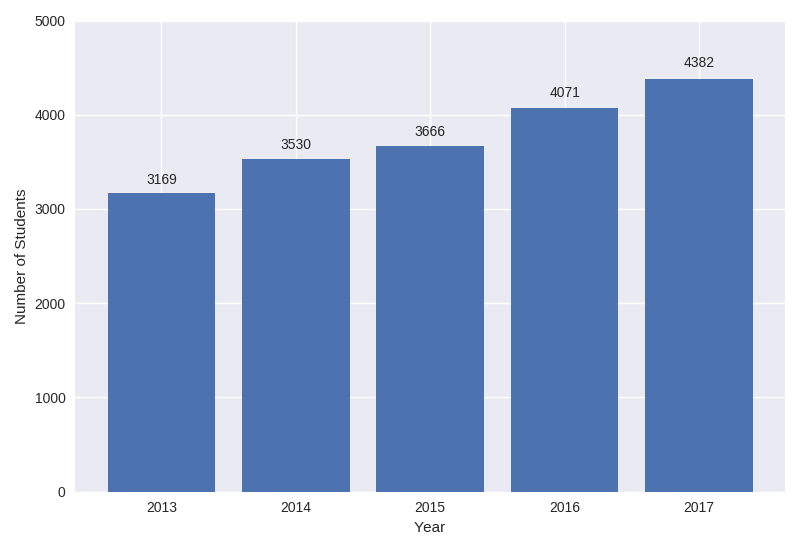
\includegraphics[width=\textwidth]{enrollment}
\caption[Enrollment at University of Waterloo]{The number of students enrolled in the Computer Science, Computer Engineering, or Software Engineering programs at the University of Waterloo continues to rise over the years \cite{uwaterloo-enrollment}.}
\label{fig:intro-enrollment}
\end{figure}

With such large classes, it becomes near-impossible to manually mark every assignment. In the past, hiring more markers was a temporary fix to this growing problem. However, this solution does not scale well because of the increased collaboration needed between markers to ensure consistency in marking. This is especially important for subjective criteria like code style that often has no \textquote{correct} answer. While marker inconsistency may be mitigated by rubrics to some extent, it still requires a deep understanding between markers.

As a result, programming assignments are generally not manually marked until the upper years where class sizes are only a couple dozen students. In rare cases, popular upper-year programming courses such as ECE459, a concurrency programming course, have hundreds of students.

Historically in ECE459, a marker would first compile and run the student's program, aided with an automated script, to eliminate trivial failures such as failed compilations or incorrect output. The marker would then manually inspect the code to check for correct usage of concurrency constructs.

One of the most common complaints amongst past markers for this course was that manually reviewing code is extremely tedious. In addition, manual marking can be error-prone because student code can greatly vary and can be hard to reason through.

%------------------------------------------------------------------------------
\section{Motivating Examples}
\label{sec:intro-motivating-examples}
%------------------------------------------------------------------------------

For the purpose of building a prototype automated marking tool, we focus our efforts on two assignments from ECE459 (see Figure~\ref{fig:intro-nonblockingio} and Figure~\ref{fig:intro-parallelprocessing}) \cite{uwaterloo-ece459}. In these assignments, the students have been provided with a working serial version of a program written in C. The program is a client that calls a web server using the cURL library. The web server, after a random delay, returns a random fragment of an image. The client program then repeats the process until it has received all the fragments. It then stitches them together to reconstruct the original image. Since the web server is on campus, the response time without the delay is usually under 20 ms. We add a Gaussian random delay to simulate network lag and prevent student programs from overwhelming the server. The students are tasked to rewrite the client with non-blocking IO constructs from the cURL library \cite{lib-curl} and again with parallelism constructs from the Pthread library \cite{lib-pthread}. Since the output of all three programs, the reconstructed image, is exactly the same, only manual code inspection can ensure students have actually fulfilled the assignment specifications.

In theory, a correctly parallelized algorithm should execute faster and use more CPU cores than its non-parallel counterpart. One might think that we should be able to check correctness by limiting the run time and checking CPU usage; however, there are a number of problems with this idea.

Firstly, there were always at least a dozen students in every class with poor programming habits who could correctly use the APIs but still have horrible run times. While these students should be penalized, their remark requests and complaints often deter markers from making deductions. To further avoid student complaints, the markers often err on the side of caution and give students a generous timeout limit that even non-parallel algorithms can pass.

Secondly, if malicious students knew that we were checking for CPU usage, they could potentially create fake threads that busy-wait to run alongside the unmodified serial algorithm.

Thirdly, due to the network delay and the possibility of receiving duplicate fragments, a program could potentially take an unpredictably long time before it can reconstruct the final image. 

Therefore, solely relying on automated input/output testing in addition to limiting the runtime or checking CPU usage in this course is insufficient to fully assess students' ability to correctly use the concurrency constructs.

\begin{figure}
\lstinputlisting[language=C, escapechar=]{../media/code/paster_nbio.c}
\caption[Non-Blocking IO Assignment]{The Non-Blocking IO assignment requires rewriting the serial program to use non-blocking  calls in the cURL library. This sample solution shows the key parts of the program that a human marker would look at, such as the cURL library function calls, and their relation to control-flow constructs, such as while-loops and if-statements.}
\label{fig:intro-nonblockingio}
\end{figure}

\begin{figure}
\lstinputlisting[language=C, escapechar=]{../media/code/paster_parallel.c}
\caption[Parallel Processing Assignment]{The Parallel Processing assignment requires the use of parallelism provided by the Pthread library. This assignment is slightly simpler than the Non-Blocking IO assignment because the student simply has to move the key components of the serial program into an isolated function that is then passed to \texttt{pthread\_create}. In this assignment, the marker has to check for the correct usage of \texttt{pthread\_*} functions and ensure proper shared memory protection with mutexes.}
\label{fig:intro-parallelprocessing}
\end{figure}

%------------------------------------------------------------------------------
\section{Approach}
%------------------------------------------------------------------------------

As described in Section~\ref{sec:intro-motivating-examples}, the manual work for markers is straightforward and checklist-like. Our goal is to encode these steps into an automated program to reduce the time needed for marking. It is important to note that we are already automating the compilation and execution of student programs to check for trivial failures (e.g. failed compilations or segmentation faults); our ultimate goal is to further augment this step to also include automated code inspection.

We hypothesize that the ASTs for correct solutions tend to be more similar to each other than incorrect solutions. The intuition behind our idea is that, in the context of programming assignments, there are a limited number of ways to effectively use the concurrency constructs. We assume students will not purposely spend excessive and unnecessary amounts of time to obscure their code or deviate from the standard code examples from class or from online tutorials.

As a result, markers generally look at certain library function calls with relation to the program structure and skim over everything else. For example, to check for correct usage in the Parallel Processing assignment (Figure~\ref{fig:intro-parallelprocessing}), a marker would check to see if \texttt{pthread\_create} and \texttt{pthread\_join} are inside loops but are not in the same loop. They would generally ignore the rest of the boilerplate code such as parameter validation and garbage collection.

From this idea, we built the ClangAutoMarker tool to automate the manual code inspection step of marking. As its name implies, this tool is built on top of the Clang and LLVM infrastructure \cite{lib-llvm}. It first leverages the Clang front-end to parse a student solution and an instructor-provided reference solution into their respective ASTs. It then post-processes these tree data structures and computes the tree edit distance\footnote{A tree $T_1$ can be converted to another tree $T_2$ through a series of steps (i.e. add, remove, or rename nodes in $T_1$ until it is equal to $T_2$). Each step also has an associated cost through a cost function $F$. The tree edit distance is the series of steps that would result in the minimum net cost to convert $T_1$ into $T_2$.} between the student solution's AST and the reference solution's AST. We then repeat this process for all the reference solutions; there are multiple reference solutions because most programming assignments have multiple valid approaches. Finally we normalize and aggregate the edit distances into a single mark between 0 to 100 for the student.

However in practice we would only accept an automated mark if it was a full mark of 100; we require manual review for assignments that did not receive full marks because these automated deductions do not have meaningful feedback relevant for a student, other than the fact that they were notably different from the reference solutions. 

This distinction does not significantly hinder the effectiveness of our tool because, traditionally, the course staff of ECE459 perfers to have a large number of students getting full marks despite having minor or benign problems with their code.

\cleardoublepage

\section{ClangAutoMarker}

%----------------------------------------------------------------------
% Simplifying the AST
%----------------------------------------------------------------------

\subsection{Simplifying the AST}

\begin{frame}{Simplifying the AST}
\begin{itemize}
\item Mimic judgement process of human reader
\item Canonicalize logically similar structures
\end{itemize}
\end{frame}

\note{
\begin{itemize}
\item The first step after we let Clang parse the solution files into an AST is to simplify it
\item This serves two purposes
\begin{itemize}
\item First it tries to mimic the judgement process of a human reader
\item Second it canonicalize logically similar structures together so that even if they are written differently and get parsed into different AST, after similification their edit distance will be minimal if not 0
\end{itemize}
\end{itemize}
}

%----------------------------------------------------------------------

\begin{frame}{If-Statements}
\begin{overprint}
\onslide<1>
\lstinputlisting[language=C]{../media/code/simplify-if-neg-before.c}

\note{
\begin{itemize}
\item Let's start with a basic example: the if-statement
\item One common difference between student code, even if they are logically similar, is their condition can swap the order of true and false branches
\item Our simplification step would then canonicalize this if-statement by deleting the NOT node and flipping the
\end{itemize}
}

%----------------------------------------------------------------------

\onslide<2>
\lstinputlisting[language=C]{../media/code/simplify-if-neg-before.c}
\begin{tikzpicture}[remember picture, overlay, every to/.style={append after command={[draw=red]}}]
\draw [thick] (cross-a) to (cross-A);
\draw [latex-latex, thick, bend left, out=45, in=135] (swap-a.east) to (swap-A.east);
\end{tikzpicture}

%----------------------------------------------------------------------

\onslide<3>
\lstinputlisting[language=C]{../media/code/simplify-if-neg-after.c}
\end{overprint}
\end{frame}

\note{
\begin{itemize}
\item Here is the resulting if-statement
\item After simplification, we were able to canonicalize both this and the original form into the same AST; this greatly reduces their edit distances
\end{itemize}
}

%----------------------------------------------------------------------

\begin{frame}{Loops}
\begin{columns}
\column{0.5\textwidth}
\lstinputlisting[language=C, basicstyle=\scriptsize\ttfamily]{../media/code/simplify-loops-for-before.c}
\lstinputlisting[language=C, basicstyle=\scriptsize\ttfamily]{../media/code/simplify-loops-while-before.c}
\lstinputlisting[language=C, basicstyle=\scriptsize\ttfamily]{../media/code/simplify-loops-do-before.c}
\column{0.5\textwidth}
\lstinputlisting[language=C]{../media/code/simplify-loops-for-after.c}
\end{columns}
\end{frame}

\note{
\begin{itemize}
\item To give another example, here are 3 types of loops
\item For a human marker, they would generally skim over the loop condition and look at the contents; they are more interested that a student is looping over the CallStatement based on a condition that involves the number 5
\item As a result, our tool simplifies all 3 types, even though they are usually not logically equivalent
\end{itemize}
}

%----------------------------------------------------------------------

\begin{frame}{Variables}
\lstinputlisting[language=C]{../media/code/simplify-var.c}
\end{frame}

\note{
\begin{itemize}
\item Another thing we simplify in our AST are variables
\item Obviously we can't assume variable names across solutions are the same. Instead we opted for a simple system of canonicalizing variables into the set of function calls that read/write to them
\item In this example, since foo is on the LHS of the bar function call, we say that foo has been writen to by bar
\item Since x and y are parameters of bar, we say that they are read by bar
\item Finally, since y is passed by reference, we say that it's also written to by bar; while this isn't necessarily true, we make the worst case assumption because interprocedural analysis is both computationally expensive and complicated
\end{itemize}
}

%----------------------------------------------------------------------
% Pruning the AST
%----------------------------------------------------------------------

\subsection{Pruning the AST}

\begin{frame}{Pruning the AST}
\begin{itemize}
\item After simplification, we still have a lot of noise in our AST
\end{itemize}
\begin{overprint}
\onslide<1>
\lstinputlisting[language=C]{../media/code/pruning-useless-before.c}

\note{
\begin{itemize}
\item After simplifying and canonicalizing our AST, we still have a fair amount of junk nodes in our AST
\item For example, a human marker would not care about the implicit casts that a parser generates
\item As a result, we then need to postprocess our AST by deleting these useless nodes
\end{itemize}
}

%----------------------------------------------------------------------

\onslide<2>
\lstinputlisting[language=C]{../media/code/pruning-useless-before.c}
\begin{tikzpicture}[remember picture, overlay, every to/.style={append after command={[draw=red]}}]
\draw [thick] (cross-a) to (cross-A);
\draw [thick] (cross-b) to (cross-B);
\end{tikzpicture}

%----------------------------------------------------------------------

\onslide<3>
\lstinputlisting[language=C]{../media/code/pruning-useless-after.c}

\end{overprint}
\end{frame}

\note{
\begin{itemize}
\item Ultimately our goal is to distill our ASTs down to their barebones skeleton that capture the structure of our original solutions
\end{itemize}
}

%----------------------------------------------------------------------
% Computing TED
%----------------------------------------------------------------------

\subsection{Computing Tree Edit Distance}

\begin{frame}{Computing Tree Edit Distance}
\begin{block}{Tree Edit Distance (TED)}
The minimum total cost of the steps needed to change from a source tree to a destination tree.
\end{block}
\end{frame}

\note{
\begin{itemize}
\item Once we finished processing our AST, we can then move on to programatically compare them
\item The algorithm we will use is the Tree Edit Distance algorithm
\item This essentially calculates the minimum cost of the steps needed to change from a source tree to a destination tree
\end{itemize}
}

%----------------------------------------------------------------------

\begin{frame}{TED Example}
\begin{center}
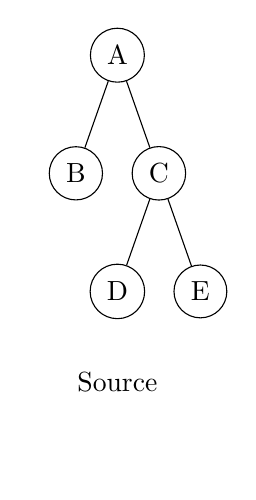
\begin{tikzpicture}[sibling distance=3em, every node/.style = {shape=circle, draw, align=center}]]
  \node{A}
    child { node{B} }
    child { node{C}
      child { node{D} }
      child { node{E} }
    }
    ;
  \node [below=3cm, align=flush center, text width=2cm, draw=none]{Source};
\end{tikzpicture}
\hspace{4em}
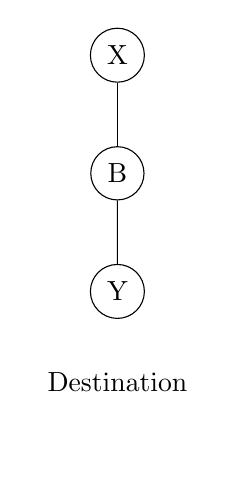
\begin{tikzpicture}[sibling distance=3em, every node/.style = {shape=circle, draw, align=center}]]
  \node{X}
    child { node{B}
      child { node{Y} }
    }
    ;
  \node [below=3cm, align=flush center, text width=2cm, draw=none]{Destination};
\end{tikzpicture}
\end{center}
\end{frame}

\note{
\begin{itemize}
\item Here is an example of how TED works
\item On the left is our source tree; on the right is our destination tree
\item In practice, these could be the student AST and reference AST
\end{itemize}
}

%----------------------------------------------------------------------

\begin{frame}{TED Example}{Delete}
\begin{center}
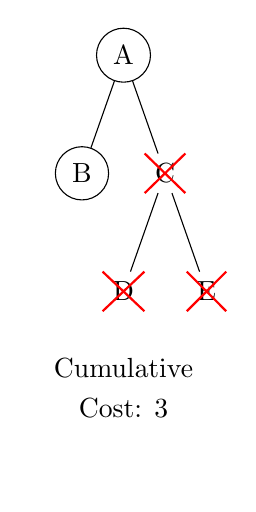
\begin{tikzpicture}[sibling distance=3em, every node/.style = {shape=circle, draw, align=center}]]
  \node{A}
    child { node{B} }
    child { node[draw=red, cross out, thick]{C}
      child { node[draw=red, cross out, thick]{D} }
      child { node[draw=red, cross out, thick]{E} }
    }
    ;
  \node [below=3cm, align=flush center, text width=2cm, draw=none]{Cumulative Cost: 3};
\end{tikzpicture}
\hspace{4em}
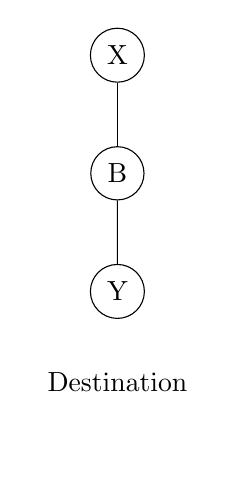
\begin{tikzpicture}[sibling distance=3em, every node/.style = {shape=circle, draw, align=center}]]
  \node{X}
    child { node{B}
      child { node{Y} }
    }
    ;
  \node [below=3cm, align=flush center, text width=2cm, draw=none]{Destination};
\end{tikzpicture}
\end{center}
\end{frame}

\note{
\begin{itemize}
\item One type of operation the TED algorithm will try is deleting existing nodes
\item The first step the algorithm might try is deleting the C,D,E nodes. Since we deleted 3 nodes, our cumulative cost thus far is 3
\item It is important to note that the cost can be varied
\item For example, we can penalize deleting variable nodes because it indicates that they are using excessive more variables than necessary
\end{itemize}
}

%----------------------------------------------------------------------

\begin{frame}{TED Example}{Insert}
\begin{center}
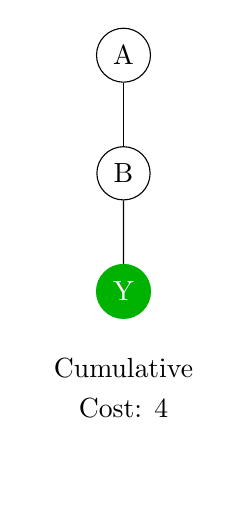
\begin{tikzpicture}[sibling distance=3em, every node/.style = {shape=circle, draw, align=center}]]
  \node{A}
    child { node{B} 
	  child { node[fill=black!30!green, draw=black!30!green, text=white]{Y} }    
    }
    ;
  \node [below=3cm, align=flush center, text width=2cm, draw=none]{Cumulative Cost: 4};
\end{tikzpicture}
\hspace{4em}
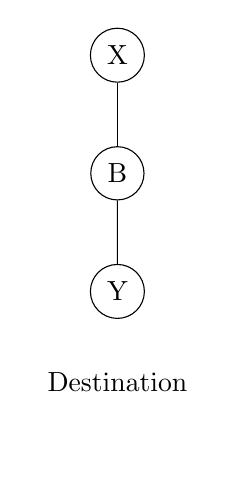
\begin{tikzpicture}[sibling distance=3em, every node/.style = {shape=circle, draw, align=center}]]
  \node{X}
    child { node{B}
      child { node{Y} }
    }
    ;
  \node [below=3cm, align=flush center, text width=2cm, draw=none]{Destination};
\end{tikzpicture}
\end{center}
\end{frame}

\note{
\begin{itemize}
\item The next type of operation is inserting new nodes
\item In our example, the algorithm then tries to insert a Y node increasing our cumulative cost to 4
\item In practice, we can for change the cost for inserting key function call nodes, meaning the student forgot to make these function calls themselves
\end{itemize}
}

%----------------------------------------------------------------------

\begin{frame}{TED Example}{Rename}
\begin{center}
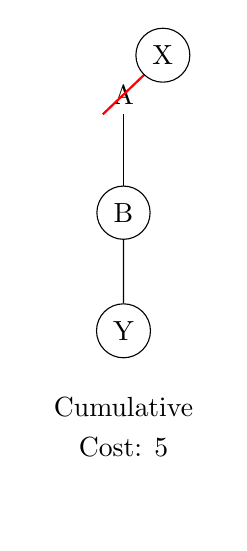
\begin{tikzpicture}[sibling distance=3em, every node/.style = {shape=circle, draw, align=center}]]
  \node[strike out, draw=red, thick](a){A}
    child { node{B} 
	  child { node{Y} }    
    }
    ;
  \node at ([yshift=0.5cm, xshift=0.5cm]a) {X};
  \node [below=3cm, align=flush center, text width=2cm, draw=none]{Cumulative Cost: 5};
\end{tikzpicture}
\hspace{4em}
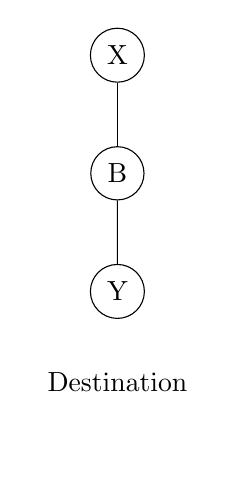
\begin{tikzpicture}[sibling distance=3em, every node/.style = {shape=circle, draw, align=center}]]
  \node{X}
    child { node{B}
      child { node{Y} }
    }
    ;
  \node [below=3cm, align=flush center, text width=2cm, draw=none]{Destination};
\end{tikzpicture}
\end{center}
\end{frame}

\note{
\begin{itemize}
\item Finally to get our destination tree, the algorithm can also rename existing nodes
\item Here we see that the total cumulative cost is 5
\end{itemize}
}


\cleardoublepage

\section{Conversion to Mark}

%----------------------------------------------------------------------
% Cutoffs
%----------------------------------------------------------------------

\subsection{Minimum Distance}

\begin{frame}{Normalized Distance}
\begin{itemize}
\item Need to normalize distances before processing
\end{itemize}
\begin{align*}
\begin{matrix}
\text{Student 1} \\
\text{Student 2} \\
\vdots \\
\text{Student $N$}
\end{matrix}
\hspace{1em}
&
\begin{bmatrix}
    T_{1,1} & T_{1,2} & T_{1,3} & \dots  & T_{1,M} \\
    T_{2,1} & T_{2,2} & T_{2,3} & \dots  & T_{2,M} \\
    \vdots & \vdots & \vdots & \ddots & \vdots \\
    T_{N,1} & T_{N,2} & T_{N,3} & \dots  & T_{N,M}
\end{bmatrix}
\end{align*}
\end{frame}

\note{
\begin{itemize}
\item Now that we have obtained our TED between each pair of student and reference solution, we then need to normalize them before we can move on to computing a final mark
\item Because each reference solution is slightly different, their resulting edit distance to each student will also be slightly different and will be in different ranges
\begin{itemize}
\item For example, reference solution 1 (first column) may range edit distances from 0 to 1000 whereas reference solution $j$ may range from 0 to 600
\end{itemize}
\item As a result, we use normalized each column with the MaxAbsScaler algorithm from the SKLearn library
\begin{itemize}
\item This normalizes each column to be between 0 to 1
\end{itemize}
\end{itemize}
}

%----------------------------------------------------------------------

\subsection{Cutoffs}

\begin{frame}{Cutoffs}
\begin{itemize}
\item Round up our computed score before giving mark back to students
\[
  \text{Mark}_i =
  \begin{cases}
    \text{Score}_i & \text{if Score$_i$ $<$ Cutoff} \\
    100            & \text{if Score$_i$ $\geq$ Cutoff}
  \end{cases}
\]
\item Designated for manual marking if Mark$_i$ is not 100
\item False positive if real mark is $<90$ but scored above cutoff
\end{itemize}
\end{frame}

\note{
\begin{itemize}
\item Before I start dicussing the actual algorithms we used to convert TED into marks, I'll first mention that we actually round up our computed scores before giving the mark back to the student
\item The main reason for this is that our tool does not currently provide meaningful/actionable feedback for the students. Students generally dislike deductions without explainations (or deductions in general!)
\begin{itemize}
\item Minor deductions from TA/our tool are usually small beign errors that are made depending on the marker's mood
\item After rounding up to 100, we say that these full-mark solutions have been automated and leave the rest for manual marking. This is generally fine for courses like ECE459 where most students are expected to receive full marks
\end{itemize}
\item In addition, we say that an automated mark is a false positive if their real mark from human marker (based on historical data) is much lower than their automated mark
\end{itemize}
}

%----------------------------------------------------------------------
% Always Full Marks
%----------------------------------------------------------------------

\subsection{Always Full Marks}

\begin{frame}{Always Full Marks}{Baseline \textquote{automated} approach to compare against}
\begin{center}

\includegraphics[scale=0.6]{presentation/always-full-marks}
\end{center}
\end{frame}

\note{
\begin{itemize}
\item First we need a baseline to compare against
\item The most obvious solution is to simply give everyone a 100. This is an "automated" approach
\end{itemize}
}

%----------------------------------------------------------------------
% Minimum Dist
%----------------------------------------------------------------------

\begin{frame}{Minimum Normalized Distance}
\begin{itemize}
\item Similar solutions should have lower TED
\item Solutions similar to reference solutions get better marks
\end{itemize}
\begin{align*}
\text{Score}_i = 100 \cdot (1 - \min\{ T'_{i,1}, T'_{i,2}, \hdots, T'_{i,M} \})
\end{align*}
\end{frame}

\note{
\begin{itemize}
\item The first approach we tried to combine TED into marks is simply using the minimum distance
\item In my original hypothesis, I said that similar solutions should have lower TED. If a student and reference solution are similar, then they would in theory have low TED
\item This formula is our first attempt at calculating a mark
\begin{itemize}
\item We do 1 minus min TED because the TED are normalized between 0 to 1, 0 being identical to reference solution
\item We multiply by 100 because marks are between 0 to 100
\end{itemize}
\end{itemize}
}

%----------------------------------------------------------------------
% Clustering
%----------------------------------------------------------------------

\subsection{Clustering}

\begin{frame}{Clustering}
\begin{itemize}
\item \textbf{Assume:} unique approaches should have similar features with each other
\item Since most students are expected to receive full marks, most solutions clusters should consist of full marks solutions
\item The volume of full-mark solutions should gravitate the centroid towards \textquote{areas} indicative of correct solutions
\begin{itemize}
\item The closer a student is to the centroid, the higher their mark
\item Score based on parameters of clustering algorithm
\end{itemize}
\end{itemize}
\end{frame}

\note{
\begin{itemize}
\item The next approach we tried was using clustering algorithms like K-Means/Gaussian Mixture/HDBSCAN
\item The basis for this approach is based on the assumption that unique approaches should have similar features with each other (e.g. they might have edit distance of 400 with Ref1, edit distance of 200 with Ref3, etc.)
\item Since most students are expected to receive full marks, most solutions clusters should consist of full marks solutions
\item The volume of full-mark solutions should gravitate the centroid towards \textquote{areas} indicative of correct solutions
\item Therefore, the closer a student is to the centroid of a cluster, the higher their mark
\end{itemize}
}

%----------------------------------------------------------------------

\begin{frame}{K-Means Clustering}{With 4 Clusters}
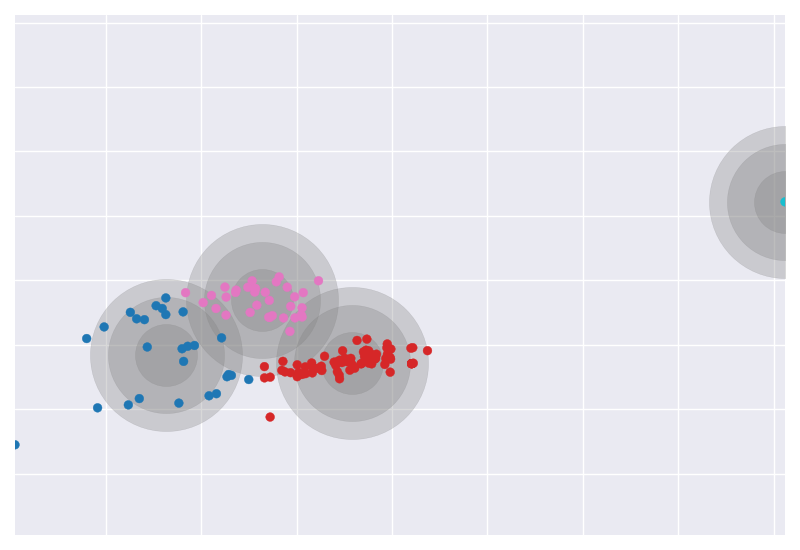
\includegraphics[width=\textwidth]{conversion-to-mark/marking_paster_nbio_ece459-a1-w2017_km}
\end{frame}

\note{
\begin{itemize}
\item That explaination was a bit of a mouthful so now let's take a look at a visual example
\item This graph visualizes the students clustered with K-Means algorithm
\begin{itemize}
\item Each unique color is a unique cluster
\item The concentric circles simply visualizes distance from the centroid
\end{itemize}
\item I dug up the outlier student in the far right
\begin{itemize}
\item Turns out he was the only student in the entire class that used epoll instead of what we told them to use: select or curl multi select (epoll is a newer standard intended to replace select)
\end{itemize}
\end{itemize}
}

%----------------------------------------------------------------------

\begin{frame}{K-Means Clustering}{Full-Marks Highlighted}
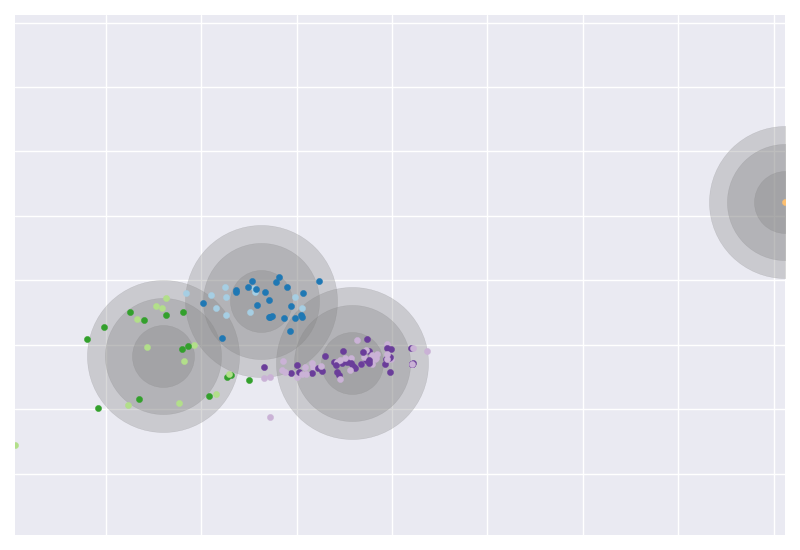
\includegraphics[width=\textwidth]{conversion-to-mark/marking_paster_nbio_ece459-a1-w2017_km_highlight}
\end{frame}

\note{
\begin{itemize}
\item This diagram highlights the students that received full-marks (from human marker) in the darker colors
\item This seems to confirm our hypothesis that clusters' centroid gravitate towards full-mark solutions
\end{itemize}
}

%----------------------------------------------------------------------
% Comparison
%----------------------------------------------------------------------

\subsection{Experimental Results}

\begin{frame}{Experimental Results}
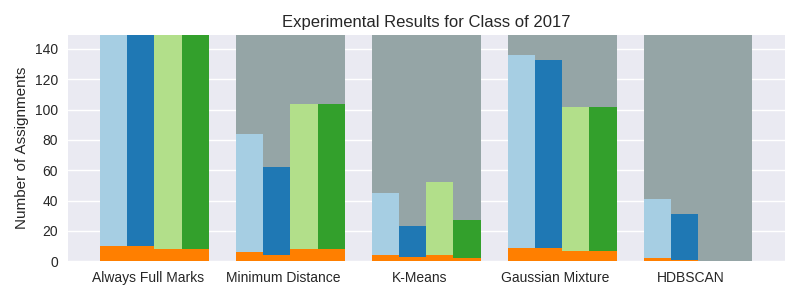
\includegraphics[width=\textwidth]{bar_triple_results_2017_3} \\
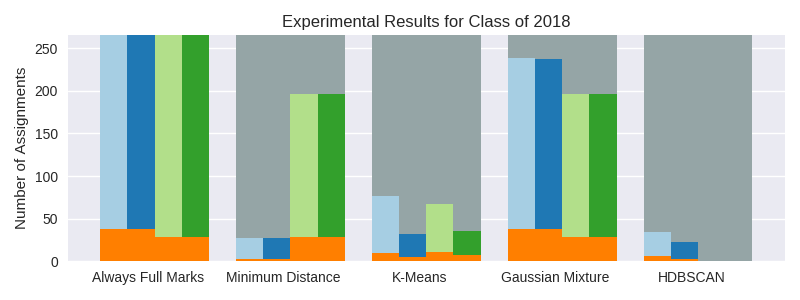
\includegraphics[width=\textwidth]{bar_triple_results_2018_3}
\end{frame}

\note{
\begin{itemize}
\item Finally we can now discuss the experimental results
\begin{itemize}
\item The blue bars represent non-blocking IO solutions; green bars represent pthreads solutions; the darker shade is cutoff at 95, and lighter shade is cutoff at 90
\item The grey bars represent assignments that were automatically graded too low (below cutoffs) and had to be manually marked
\item The orange bars represent the false positives
\end{itemize}
\item
\begin{itemize}
\item We see that K-Means and HDBSCAN are ineffective because their automation rates are too low; then again if we're expecting as many students to receive full marks then they are pretty decent because their false positives are the lowest
\item The MinDist and GM have higher automation rate and false positives; the squashed bars make it look worse than it actually is but regardless the false positive rate is a bit too close to the AlwaysFull
\end{itemize}
\end{itemize}
}

%----------------------------------------------------------------------

\begin{frame}{Shortcomings}{Noise in AST}
\begin{itemize}
\item More edge cases to consider
\item Only looked at correct solutions for clustering features
\end{itemize}
\end{frame}

\note{
\begin{itemize}
\item Clearly our results were not as great as we originally had hoped. As a result, we went back to look at our shortcomings
\item Once we tested our tool with the entire class rather than just a small subset of cases, we found a lot more edge cases to consider
\begin{itemize}
\item For example, there are a few students that wrote their loops to be: while(true) if cond break
\item Had I realized this case eariler, I would have canonicalized loops simply track conditions that break out of them
\end{itemize}
\item Another problem is that we only looked at correct reference solutions for clustering features
\begin{itemize}
\item In a similar related work, the authors mentioned that their false positives went down when their reference solutions also included incorrect solutions
\item Unfortunately since most students are expected to receive full marks, we do not have enough data for "incorrect solutions"
\end{itemize}
\end{itemize}
}

%----------------------------------------------------------------------

\begin{frame}{Shortcomings}{Uncertain ground truth}
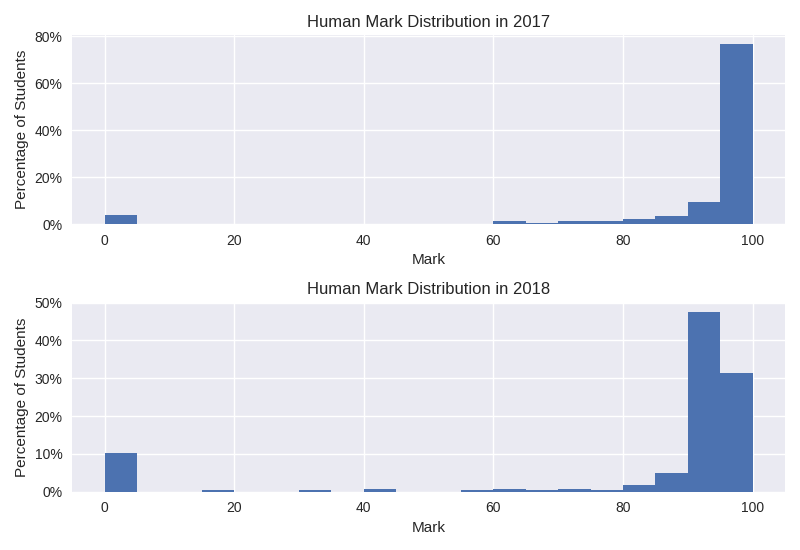
\includegraphics[width=\textwidth]{human_marks}
\end{frame}

\note{
\begin{itemize}
\item Another shortcoming is that we are also uncertain about the validity of our ground truth data
\item We see that there is a discrepency in marker leniency between the 2 classes
\item This brings into question whether human markers are as infallible as we originally assumed
\item Furthermore, we also need to consider that the ground truth mark data includes deductions unrelated to their code: late days deductions, mistakes in their report, etc.
\end{itemize}
}

%----------------------------------------------------------------------

\begin{frame}{Shortcomings}{Uncertain ground truth}
\begin{itemize}
\item Remarked subset of assignments to use as ground-truth
\end{itemize}

\begin{table}
\resizebox{\linewidth}{!}{%
\begin{tabular}{lrrrr} \toprule
\multirow{2}{*}{}
& \multicolumn{2}{c}{2017 Class} & \multicolumn{2}{c}{2018 Class}  \\
& Automated & False Positives & Automated & False Positives  \\
\midrule
Always Full Marks & 20 & 2 & 20 & 7 \\
Min Distance      & 5  & 0 & 1  & 0 \\
K-Means           & 2  & 0 & 2  & 0 \\
Gaussian Mixture  & 8  & 0 & 14 & 3 \\
HDBSCAN           & 0  & - & 0  & - \\
\bottomrule
\end{tabular}
}
\end{table}
\end{frame}

\note{
\begin{itemize}
\item As a result, I've faithfully remarked a subet of assignments to use as ground-truth
\item We see that the automation rate is relatively consistent with our initial result so this is a good random sample
\item We also see that the false positives have significantly dropped with the new ground truth 
\end{itemize}
}

\cleardoublepage

\chapter{Related Works}
\label{chap:related-works}

Writing programs is one method used in computer science education to reinforce and assess practical concepts taught in class. Automating the manual marking process has been a widely studied topic due to the need for quick feedback turnaround and, by removing or minimizing the human element, maximizes objectivity and consistency. This chapter explores several tools in this field; since there are too many tools to count, we will mainly focus on tools designed for interoperability rather than ones designed for niche domains or specific assignments.

%--------------------------------------------------------------------------------
\section{Input/Output Marking}
%--------------------------------------------------------------------------------

The earliest published example we found of automated programming assignment marking dates back to 1989 by Isaacson and Scott \cite{isaacson1989automating}. Their approach is one of the most common automated marking techniques used in practice today: they compile each student's program (if possible), execute the students' programs with input files, and compare the programs' outputs with expected output files. This process is straightforward and easy-to-understand for testing program functionality. There are many subsequent works \cite{cheang2003automated, higgins2003coursemarker, jackson1997grading, morris2003automatic, spacco2006experiences} that further enhance their process. These tools ultimately all follow the same three steps.

%--------------------------------------------------------------------------------
\section{Fill-In-The-Gap Marking}
%--------------------------------------------------------------------------------

Another increasingly common assignment style and marking technique is called \textquote{fill-in-the-gap}. As this name implies, these assignments provide students with gaps in instructor-provided template code to fill prior to compilation and analysis. For example, an instructor might provide students with a method signature for a binary search algorithm and task them to implement the algorithm itself. Lieberman \cite{lieberman1986example} has stated that this assignment style is the most effective way for beginner programmers to apply newly-taught concepts. Due to the rigid nature of these assignment specifications and extremely small analysis space, many static analysis techniques have been developed to analyze these gaps.

The Environment for Learning to Program (ELP) marking platform developed by Truong et al. \cite{truong2004static} is an example of the fill-in-the-gap assignment style used in practice. After a student submits their assignment, their tool compiles the student program and extracts the relevant \textquote{gap} from the resulting AST for later analysis. Similar to our tool, they also perform some AST normalization prior to analysis in order to minimize the amount of variety among functionally-similar programs. After extracting the gaps, they perform analysis such as checking variable states and invariants before/after gaps and metrics such as line-length and cyclomatic complexity.

OverCode developed by Glassman et al. \cite{glassman2015overcode} is another marking platform based on the idea of fill-in-the-gap style Python programming assignments in Massive Open Online Courses (MOOC). They first clean up student programs such as normalizing variable names. They then cluster student solutions based on line-by-line comparison such that programs with similar lines are in the same clusters. The resulting clusters are presented to instructors to manually provide feedback and scores. We note that their approach was mainly made possible due to the simplicity of Python and of the assignment specification as well as the massive amount of submission data available to analyze. In offline classes such as the class we analyzed with only hundreds of students, rather than tens of thousands, it is unlikely their approach will be able to extract meaningful-sized clusters for analysis.

The disadvantage of these types of assignments and their corresponding tools is that they are mostly used in beginner programming classes rather than upper-year classes, such as the one analyzed in this thesis. Furthermore, they do not score student assignments beyond input/output testing; however, it is theoretically possible for them to apply a score based on their static analysis results such as applying deductions for high cyclomatic complexity. Nonetheless, advanced programming assignments such as our Non-Blocking IO and Parallel Processing assignments are more open-ended and generally consist of significantly larger non-divisible methods that are not as easily analyzable by the aforementioned tools.

%--------------------------------------------------------------------------------
\section{AST-Based Marking}
%--------------------------------------------------------------------------------

There are many prior works exploring the idea of automatically comparing student solutions to reference solutions at the solution level using ASTs. One common element found in all of these works is the need for normalizing ASTs by collapsing functionally-similar substructures into canonical forms prior to analysis. This is essential to reducing the number of distinct solutions to analyze and avoiding falsely penalizing functionally-similar code. In addition to the field of automated program marking, normalizing AST substructures is widely studied in other fields such as plagiarism and clone detection \cite{baxter1998clone, feng2013code}.

Singh et al. \cite{singh2013automated} developed an error-correction language for describing steps to transform an incorrect student solution into a correct reference solution. In addition to reference solutions, the instructor must also describe common student errors and the steps to correct them using the error-correction language. Their system then utilizes a constraint solver to find the minimum steps needed to correct the student solutions. Finally, it scores the student based on the steps. This is similar to our tool's cost model described in Section~\ref{sec:cam-cost-model} where we associate a cost for any change to be made to the student AST.

Thorburn and Rowe's PASS tool \cite{thorburn1997pass} also requires additional work from the instructors prior to scoring students. Their tool requires the instructor to specify an hierarchical \textquote{solution plan} for each assignment; this is essentially a breakdown of the steps to solve a problem. For example, a merge sort problem consists of a \textquote{sort} function at the top level; it then consists of sub-components such as checking the base case, pivoting the input, and the making two recursive calls. Their tool attempts to find equivalent program components in the student code. They check for equivalence by comparing component outputs when given randomly generated inputs. Students are then scored based on the number of equivalent components found.

The main drawback for both Singh et al.'s and Thorburn and Rowe's tools is the additional work needed for instructors beyond providing reference solutions. Singh et al.'s work requires instructors to anticipate and describe common errors and corrections in a custom language. This may prove difficult as one cannot anticipate all possible errors a student may make. Thorburn and Rowe's work requires instructors to describe a solution plan by hierarchically breaking down a problem into smaller sub-problems. This may not always be possible for every assignment as some assignments may have large indivisible components.

AssignSim developed by Naud\'e et al. \cite{naude2010marking} was perhaps the most similar prior work to ours. Their tool directly compares solution ASTs and generates a score based on their similarities. Our works differ in how we compare the post-processed ASTs and score the student. They generate scores by directly analyzing the graphs and assigning scores based on the differing nodes and their respective neighbour nodes. On the other hand, our work utilizes a generic tree edit distance algorithm to compare the graphs and then aggregate the various edit distances into a mark. Their results were slightly better than ours when their set of reference solutions contained both high quality and low quality solutions (i.e. both high marks and low marks). However, when they only had high quality solutions, their accuracy fell to similar levels as ours. This led us to speculate that our choice of reference solutions (only high marks) may also had an influence in our results; however since the majority of past students in our data set have received full marks, we do not have sufficient data to pursue further investigation.

\cleardoublepage

\chapter{Conclusion}
\label{chap:conclusion}

This thesis presented a novel approach to automatically mark programming assignments. Our approach consists of two components: (1) we first prune a program's AST to isolate key features relevant for assignment marking; (2) we then compare a student solution to a set of reference solutions in order to generate a final mark for the student. Assignments that have received automated deductions will require manual review to provide more meaningful and individualized feedback.

This tool assumes the majority of the students will write their programs in specific patterns. We are concerned this may limit student creativity when trying to solve their assignments. However, we note that the programming assignments we tested with had rigid designs and the easiest-to-implement solutions often fall under specific patterns. Therefore we do not believe this to be a major concern.

We implemented our processes as the ClangAutoMarker tool and tested it with student submissions and marks from previous offerings of the ECE459 course at the University of Waterloo. Our initial results were not as successful as we had originally hoped. Our tool did not perform better than the baseline approach of simply always assigning full marks. However, due to the uncertainty in our ground-truth, we faithfully recollected the ground-truth data for a smaller subset of previous classes. When we reevaluated our tool with the more accurate sample, we were able to achieve a better false positive rate of 21\% compared to always assigning full marks which had a false positive rate of 35\%. Although this was still not very accurate, we have demonstrated that our tool has promising potential for automated marking and further improvements may make it viable for a live classroom.

\cleardoublepage

%------------------------------------------------------------------------------
% Bibliography
%------------------------------------------------------------------------------

\bibliographystyle{plain}

\cleardoublepage % This is needed if the book class is used, to place the anchor in the correct page,
                 % because the bibliography will start on its own page.
                 % Use \clearpage instead if the document class uses the "oneside" argument

\phantomsection  % With hyperref package, enables hyperlinking from the table of contents to bibliography

% The following statement causes the title "References" to be used for the bibliography section:
\renewcommand*{\bibname}{References}

% Add the References to the Table of Contents
\addcontentsline{toc}{chapter}{\textbf{References}}

\bibliography{thesis}
\cleardoublepage

%------------------------------------------------------------------------------
% Back Matter
%------------------------------------------------------------------------------

\appendix

\chapter{Results of Scoring Algorithms}

This appendix contains the tables presenting the results of each tree edit distance scoring method we presented in Chapter~\ref{chap:ctm}.

Assignments were considered \textquote{Automatable} if they scored higher than certain cutoff points. For these assignments, we analyzed their false positive rate; this was the percentage of assignments that scored higher than what they had originally earned from a human marker. Conversely, if an assignment scored lower than certain cutoff points or triggered processing errors due to unexpected AST structures or assertion failures, then it was designated for manual marking because we wanted to provide meaningful feedback to students for any deductions that they receive. 

\begin{table}
\caption{Always Assigning Full Marks}
\label{tab:ctm-full-marks}
\begin{tabular}{lrrrr} \toprule
& \multicolumn{2}{c}{2017} & \multicolumn{2}{c}{2018} \\
& 90 Cutoff & 95 Cutoff & 90 Cutoff & 95 Cutoff \\
\midrule
\multicolumn{5}{l}{ \textbf{Non-Blocking IO Assignment} }\\
\tspace Total Students           &   149 &   149 &   265 &   265 \\
\tspace Non Automatable          &     0 &     0 &     0 &     0 \\
\tspace \tspace Below Cutoff     &     0 &     0 &     0 &     0 \\
\tspace \tspace Processing Error &     0 &     0 &     0 &     0 \\
\tspace Automatable              &   149 &   149 &   265 &   265 \\
\tspace \tspace False Positives  &    10 &    10 &    38 &    38 \\
\\
\multicolumn{5}{l}{ \textbf{Parallel Processing Assignment} }\\
\tspace Total Students           &   149 &   149 &   265 &   265 \\
\tspace Non Automatable          &     0 &     0 &     0 &     0 \\
\tspace \tspace Below Cutoff     &     0 &     0 &     0 &     0 \\
\tspace \tspace Processing Error &     0 &     0 &     0 &     0 \\
\tspace Automatable              &   149 &   149 &   265 &   265 \\
\tspace \tspace False Positives  &     8 &     8 &    29 &    29 \\
\bottomrule
\end{tabular}

\end{table}

\begin{table}
\caption{Using Minimum Normalized Edit Distance to Obtain Mark}
\label{tab:ctm-min-dist}
\begin{tabular}{lrrrr} \toprule
& \multicolumn{2}{c}{2017} & \multicolumn{2}{c}{2018} \\
& 90 Cutoff & 95 Cutoff & 90 Cutoff & 95 Cutoff \\
\midrule
\multicolumn{5}{l}{ \textbf{Non-Blocking IO Assignment} }\\
\tspace Total Students           &   149 &   149 &   265 &   265 \\
\tspace Non Automatable          &    65 &    87 &   238 &   238 \\
\tspace \tspace Below Cutoff     &    54 &    76 &   223 &   223 \\
\tspace \tspace Processing Error &    11 &    11 &    15 &    15 \\
\tspace Automatable              &    84 &    62 &    27 &    27 \\
\tspace \tspace False Positives  &     6 &     4 &     3 &     3 \\
\\
\multicolumn{5}{l}{ \textbf{Parallel Processing Assignment} }\\
\tspace Total Students           &   149 &   149 &   265 &   265 \\
\tspace Non Automatable          &    45 &    45 &    69 &    69 \\
\tspace \tspace Below Cutoff     &     0 &     0 &     0 &     0 \\
\tspace \tspace Processing Error &    45 &    45 &    69 &    69 \\
\tspace Automatable              &   104 &   104 &   196 &   196 \\
\tspace \tspace False Positives  &     8 &     8 &    29 &    29 \\
\bottomrule
\end{tabular}

\end{table}

\begin{table}
\caption{Using K-Means Clustering to Obtain Mark}
\label{tab:ctm-km}
\begin{tabular}{lrrrr} \toprule
& \multicolumn{2}{c}{2017} & \multicolumn{2}{c}{2018} \\
& 90 Cutoff & 95 Cutoff & 90 Cutoff & 95 Cutoff \\
\midrule
\multicolumn{5}{l}{ \textbf{Non-Blocking IO Assignment} }\\
\tspace Total Students           &   149 &   149 &   265 &   265 \\
\tspace Non Automatable          &   104 &   126 &   188 &   233 \\
\tspace \tspace Below Cutoff     &    93 &   115 &   173 &   218 \\
\tspace \tspace Processing Error &    11 &    11 &    15 &    15 \\
\tspace Automatable              &    45 &    23 &    77 &    32 \\
\tspace \tspace False Positives  &     4 &     3 &    10 &     5 \\
\\
\multicolumn{5}{l}{ \textbf{Parallel Processing Assignment} }\\
\tspace Total Students           &   149 &   149 &   265 &   265 \\
\tspace Non Automatable          &    97 &   122 &   205 &   239 \\
\tspace \tspace Below Cutoff     &    52 &    77 &   136 &   170 \\
\tspace \tspace Processing Error &    45 &    45 &    69 &    69 \\
\tspace Automatable              &    52 &    27 &    60 &    26 \\
\tspace \tspace False Positives  &     4 &     2 &    10 &     4 \\
\bottomrule
\end{tabular}

\end{table}

\begin{table}
\caption{Using Gaussian Mixture Clustering to Obtain Mark}
\label{tab:ctm-gm}
\begin{tabular}{lrrrr} \toprule
& \multicolumn{2}{c}{2017} & \multicolumn{2}{c}{2018} \\
& 90 Cutoff & 95 Cutoff & 90 Cutoff & 95 Cutoff \\
\midrule
\multicolumn{5}{l}{ \textbf{Non-Blocking IO Assignment} }\\
\tspace Total Students           &   149 &   149 &   265 &   265 \\
\tspace Non Automatable          &    18 &    23 &    40 &    52 \\
\tspace \tspace Below Cutoff     &     7 &    12 &    25 &    37 \\
\tspace \tspace Processing Error &    11 &    11 &    15 &    15 \\
\tspace Automatable              &   131 &   126 &   225 &   213 \\
\tspace \tspace False Positives  &     9 &     8 &    35 &    33 \\
\\
\multicolumn{5}{l}{ \textbf{Parallel Processing Assignment} }\\
\tspace Total Students           &   149 &   149 &   265 &   265 \\
\tspace Non Automatable          &    47 &    47 &    69 &    69 \\
\tspace \tspace Below Cutoff     &     2 &     2 &     0 &     0 \\
\tspace \tspace Processing Error &    45 &    45 &    69 &    69 \\
\tspace Automatable              &   102 &   102 &   196 &   196 \\
\tspace \tspace False Positives  &     8 &     8 &    29 &    29 \\
\bottomrule
\end{tabular}

\end{table}

\begin{table}
\caption{Using HDBSCAN Clustering to Obtain Mark}
\label{tab:ctm-hdb}
\begin{tabular}{lrrrr} \toprule
& \multicolumn{2}{c}{2017} & \multicolumn{2}{c}{2018} \\
& 90 Cutoff & 95 Cutoff & 90 Cutoff & 95 Cutoff \\
\midrule
\multicolumn{5}{l}{ \textbf{Non-Blocking IO Assignment} }\\
\tspace Total Students           &   149 &   149 &   265 &   265 \\
\tspace Non Automatable          &   108 &   118 &   231 &   242 \\
\tspace \tspace Below Cutoff     &    97 &   107 &   216 &   227 \\
\tspace \tspace Processing Error &    11 &    11 &    15 &    15 \\
\tspace Automatable              &    41 &    31 &    34 &    23 \\
\tspace \tspace False Positives  &     2 &     1 &     6 &     3 \\
\\
\multicolumn{5}{l}{ \textbf{Parallel Processing Assignment} }\\
\tspace Total Students           &   149 &   149 &   265 &   265 \\
\tspace Non Automatable          &   149 &   149 &   265 &   265 \\
\tspace \tspace Below Cutoff     &   104 &   104 &   196 &   196 \\
\tspace \tspace Processing Error &    45 &    45 &    69 &    69 \\
\tspace Automatable              &     0 &     0 &     0 &     0 \\
\tspace \tspace False Positives  &     0 &     0 &     0 &     0 \\
\bottomrule
\end{tabular}

\end{table}


\end{document}
